\documentclass[12pt]{article}

\usepackage{sbc-template}

\usepackage{graphicx,url}

%\usepackage[brazil]{babel}   
\usepackage[utf8]{inputenc}  
\usepackage{amsmath}
\usepackage{algorithm}
\usepackage{algorithmic}
\usepackage{svg}

\sloppy

\title{Análise de Algoritmos de Caminho Mínimo: Dijkstra, Min-Max e Max-Min para Gargalos}

\author{Lucas Gualtieri Firace\inst{1}, Gabriel Martins Rajão\inst{1}, Luiza Dias Corteletti\inst{1} }

\address{Instituto de Ciências Exatas e Informática - PUC Minas}

\begin{document} 

\maketitle

\begin{resumo} 
  O artigo explora três algoritmos de otimização de caminho em grafos: Dijkstra, Min-Max e Max-Min. O algoritmo de Dijkstra minimiza o custo total de um caminho, somando os pesos das arestas, enquanto os problemas Min-Max e Max-Min focam na otimização de gargalos. O Min-Max minimiza o maior gargalo, enquanto o Max-Min maximiza o menor gargalo ao longo do caminho. Esses algoritmos têm aplicações práticas em redes de comunicação e tráfego, onde a capacidade de cada aresta é um fator crítico para garantir a eficiência do fluxo.
\end{resumo}

\section{Definição dos Problemas}

Os problemas \textbf{Min-Max} e \textbf{Max-Min} para gargalos estão relacionados à otimização de caminhos em grafos, com foco nas restrições impostas por gargalos ou limitações de capacidade ao longo das arestas do grafo. Esses problemas diferem do algoritmo de Dijkstra, que visa encontrar o caminho de menor custo total. A seguir, definimos cada um deles e discutimos suas diferenças.

\subsection{Problema Min-Max de Gargalos}

O objetivo do problema \textbf{Min-Max} é encontrar um caminho em um grafo onde o \textbf{maior peso (gargalo)} das arestas seja o \textbf{menor possível}. Em outras palavras, entre todos os caminhos disponíveis de um nó de origem para um nó de destino, deve-se escolher aquele cujo peso máximo da aresta no caminho seja o menor possível.

\subsubsection{Aplicação}
Este problema é utilizado em cenários onde o maior limite de uma aresta (como a capacidade de um link) ao longo do caminho é o fator mais crítico, como em redes de fluxo de dados ou logísticas, onde deseja-se minimizar o pior cenário de congestionamento.

\subsubsection{Exemplo} Em uma rede de comunicação de dados, o problema Min-Max tentaria escolher o caminho cujo \textbf{trecho com o maior atraso (link mais lento)} seja o mais favorável. Por exemplo, se em um caminho temos links com latências de 40ms, 60ms, 80ms e 120ms, o Min-Max tentaria minimizar o caminho em que o maior atraso (120ms) fosse o menor possível, talvez escolhendo um caminho com latências de 40ms, 60ms e 80ms, onde o maior atraso seria 80ms. Dessa forma, Min-Max garante que o pior atraso entre os links no caminho escolhido seria minimizado.

\subsection{Problema Max-Min de Gargalos}

No problema \textbf{Max-Min}, o objetivo é maximizar o \textbf{menor peso (gargalo)} em um caminho. Ou seja, entre todos os caminhos disponíveis, escolhe-se o caminho cujo \textbf{menor peso da aresta (gargalo)} seja o maior possível. O foco é tentar garantir o maior gargalo mínimo ao longo de um caminho.

\subsubsection{Aplicação}
Este problema é utilizado em situações onde deseja-se maximizar a menor capacidade possível em um caminho, garantindo que o menor gargalo em um caminho seja o maior possível. Isso é importante em cenários de comunicação ou transporte, onde é essencial garantir que o caminho tenha a maior capacidade mínima possível para evitar congestionamentos.

\subsubsection{Exemplo}
Imagine uma rede de fluxo de dados em que cada aresta representa a capacidade de um link. O problema Max-Min busca o caminho onde o \textbf{link mais restritivo} (o gargalo) tenha a maior capacidade possível. Por exemplo, se em um caminho temos links com capacidades 100, 50, 30 e 70, o gargalo seria 30. O Max-Min tenta encontrar o caminho cujo gargalo seja o maior entre todos os possíveis caminhos.

\section{Diferenças em relação ao Algoritmo de Dijkstra}

O algoritmo de Dijkstra busca o \textbf{caminho de menor custo total} entre dois nós em um grafo, somando os pesos das arestas ao longo de um caminho. Já os problemas de \textbf{Min-Max} e \textbf{Max-Min} focam em \textbf{otimizar os gargalos} ao longo do caminho, não considerando o custo total do caminho, mas sim as capacidades mínimas ou máximas nas arestas.

\begin{itemize}
    \item \textbf{Dijkstra}: Foca no \textbf{custo total} do caminho, somando os pesos de todas as arestas.
    \item \textbf{Min-Max}: Minimiza o maior gargalo ao longo de um caminho.
    \item \textbf{Max-Min}: Maximiza o menor gargalo ao longo de um caminho.
\end{itemize}

Esses dois problemas são úteis em contextos onde o foco não é necessariamente minimizar a distância ou o custo total do caminho, mas sim garantir que as restrições impostas por gargalos ao longo do caminho sejam tratadas da maneira mais eficiente.

\section{Aplicações}

Esses problemas são frequentemente aplicados em \textbf{redes de comunicação, redes de tráfego ou roteamento de dados}, onde a capacidade limitada de cada enlace entre nós precisa ser considerada para garantir um fluxo eficiente.

\begin{figure}[h] % 'h' tenta posicionar a figura aqui
    \centering
    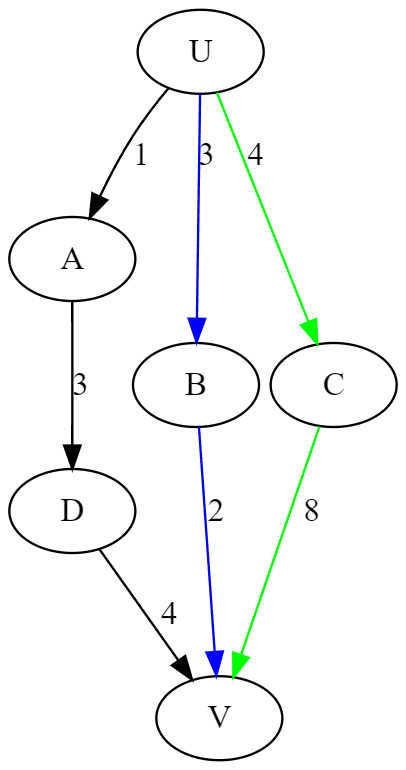
\includegraphics[width=.7\textwidth]{caminhos.png}
    \caption{Caminho em azul representa o caminho encontrado pelo algoritmo Min-Max, onde o objetivo é minimizar o maior gargalo (capacidade máxima) ao longo do caminho. Caminho em verde representa o caminho encontrado pelo algoritmo Max-Min, que busca maximizar a menor capacidade (gargalo) ao longo do caminho.}
    \label{fig:123}
\end{figure}

\newpage

\section{Algoritmo de Dijkstra}

O algoritmo de Dijkstra tem como objetivo encontrar o caminho de \textbf{menor custo total} de um vértice de origem para todos os outros vértices. Ele usa uma \textbf{fila de prioridade (min-heap)} para garantir que o próximo vértice a ser explorado tenha a menor distância acumulada até o momento. O que é propagado de um vértice para o outro é a \textbf{soma das distâncias} (ou pesos das arestas) ao longo do caminho.

\begin{itemize}
    \item A cada iteração, o vértice com a menor distância acumulada é removido da fila de prioridade.
    \item Para cada vizinho, a distância total (distância acumulada até o vértice atual + peso da aresta) é calculada.
    \item Se essa nova distância for menor que a distância registrada anteriormente para o vizinho, 
    essa distância é atualizada, e o vizinho é adicionado ou tem sua prioridade atualizada na fila.
    \item O algoritmo para assim que todos os vértices tiverem sido visitados.
\end{itemize}


\begin{algorithm}
\caption{Dijkstra's Algorithm}
\begin{algorithmic}[1]
\REQUIRE Grafo \( G(V, E) \), vértice de origem \( x \)
\ENSURE Lista de distâncias mínimas \( D \)

\STATE Inicialize o vetor de distâncias \( D[v] \leftarrow \infty \) \(\forall v \in V\)
\STATE \( D[x] \leftarrow 0 \)
\STATE Inicialize uma fila de prioridade \( Q \)
\STATE \( Q.push(x, 0) \)
\WHILE{\( Q \) não estiver vazia}
    \STATE \( u \leftarrow Q.pop() \)
     \FOR{cada \(v \in \Gamma(u)\)}
        \IF{ \( D[u] + w(u, v) < D[v] \)}
            \STATE \( D[v] \leftarrow D[u] + w(u, v) \)
            \IF{ \( v \notin Q \)}
                \STATE \( Q.push(v, D[v]) \)
            \ELSE
                \STATE Atualize a chave de \( v \) em \( Q \) para \( D[v] \)
            \ENDIF
        \ENDIF
    \ENDFOR
\ENDWHILE
\RETURN \( D \)
\end{algorithmic}
\end{algorithm}

\newpage

\section{Algoritmo Max-Min (Capacidade Máxima)}

O algoritmo Max-Min busca encontrar o caminho entre a origem e o destino de modo a \textbf{maximizar o menor gargalo (capacidade mínima) ao longo do caminho}. Ele utiliza uma \textbf{fila de prioridade (max-heap)} para sempre expandir o vértice que tem a maior capacidade mínima disponível até o momento. Aqui, \textbf{o valor propagado entre vértices é a menor capacidade (gargalo)} no caminho até o momento. O objetivo é garantir que o caminho escolhido maximize a menor capacidade entre os vértices.

\begin{itemize}
    \item A cada iteração, o vértice com a maior capacidade mínima acumulada é removido da fila.
    \item Para cada vizinho, é calculada a nova capacidade mínima, que é o menor valor entre a capacidade mínima do vértice atual e o peso da aresta que o conecta ao vizinho.
    \item Se essa nova capacidade mínima for maior que a registrada anteriormente para o vizinho, essa capacidade é atualizada, e o vizinho é adicionado ou tem sua prioridade atualizada na fila.
    \item O algoritmo para assim que vértice de destino é removido da fila.
\end{itemize}

\begin{algorithm}
\caption{Algoritmo Max-Min Path}

\begin{algorithmic}[1]
\REQUIRE Grafo \( G(V, E) \), vértice de origem \( source \), vértice de destino \( target \)
\ENSURE Caminho \( P(source, target) \) que maximiza a menor capacidade

\STATE Inicialize o vetor de predecessores \( predecessors[v] \leftarrow -1 \) \(\forall v \in V\)
\STATE Inicialize a fila de prioridade \( Q.push(v, -\infty ) \) \(\forall v \in V\)
\STATE Inicialize o vetor de capacidades minimas \( nodeCapacity[v] \leftarrow -\infty\) \(\forall v \in V\)
\STATE \( nodeCapacity[source] \leftarrow \infty \)
\STATE \( Q.push(source, \infty) \)
\WHILE{\( Q \) não estiver vazia}
    \STATE \( u \leftarrow Q.pop() \) \COMMENT{Retira o vértice com maior capacidade disponível}
    \IF{ \( u = target \)}
        \STATE \textbf{interrompemos a busca e reconstruímos o caminho}
    \ENDIF
    \FOR{cada \(v \in \Gamma(u)\)}
        \STATE \( newCapacity \leftarrow \min(nodeCapacity[u], w(u, v)) \)
        \IF{ \( nodeCapacity[v] < newCapacity \)}
            \STATE \( predecessors[v] \leftarrow u \)
            \STATE \( nodeCapacity[v] \leftarrow newCapacity \)
            \STATE Atualize a chave de \( v \) em \( Q \) para \( nodeCapacity[v] \)
        \ENDIF
    \ENDFOR
\ENDWHILE
\RETURN \texttt{constructPath(source, target, predecessors)}
\end{algorithmic}
\end{algorithm}

\newpage

\section{Algoritmo Min-Max (Capacidade Mínima)}

O algoritmo Min-Max tenta minimizar o maior gargalo possível ao longo do caminho, ou seja, \textbf{encontrar o caminho em que o maior peso das arestas seja o menor possível}. Ele usa uma \textbf{fila de prioridade (min-heap)} para garantir que o próximo vértice a ser explorado tenha o menor gargalo máximo até o momento. Neste caso, \textbf{o valor propagado entre vértices é o maior peso (gargalo)} no caminho até o momento. O objetivo é garantir que o caminho escolhido minimize o maior gargalo.

\begin{itemize}
    \item A cada iteração, o vértice com o menor gargalo máximo acumulado é removido da fila.
    \item Para cada vizinho, é calculado o novo gargalo máximo, que é o maior valor entre o gargalo máximo do vértice atual e o peso da aresta que o conecta ao vizinho.
    \item Se essa nova capacidade máxima for menor que a registrada anteriormente para o vizinho, essa capacidade é atualizada, e o vizinho é adicionado ou tem sua prioridade atualizada na fila.
    \item O algoritmo para assim que vértice de destino é removido da fila.
\end{itemize}

\begin{algorithm}
\caption{Algoritmo Min-Max Path}
\begin{algorithmic}[1]
\REQUIRE Grafo \( G(V, E) \), vértice de origem \( source \), vértice de destino \( target \)
\ENSURE Caminho \( P(source, target) \) que maximiza a menor capacidade

\STATE Inicialize o vetor de predecessores \( predecessors[v] \leftarrow -1 \) \(\forall v \in V\)
\STATE Inicialize a fila de prioridade \( Q.push(v, \infty ) \) \(\forall v \in V\)
\STATE Inicialize o vetor de capacidades maximas \( nodeCapacity[v] \leftarrow \infty\) \(\forall v \in V\)
\STATE \( nodeCapacity[source] \leftarrow \infty \)
\STATE \( Q.push(source, -\infty) \)
\WHILE{\( Q \) não estiver vazia}
    \STATE \( u \leftarrow Q.pop() \) \COMMENT{Retira o vértice com menor capacidade disponível}
    \IF{ \( u = target \)}
        \STATE \textbf{interrompemos a busca e reconstruímos o caminho}
    \ENDIF
    \FOR{cada \(v \in \Gamma(u)\)}
        \STATE \( newCapacity \leftarrow \max(nodeCapacity[u], w(u, v)) \)
        \IF{ \( nodeCapacity[v] > newCapacity \)}
            \STATE \( predecessors[v] \leftarrow u \)
            \STATE \( nodeCapacity[v] \leftarrow newCapacity \)
            \STATE Atualize a chave de \( v \) em \( Q \) para \( nodeCapacity[v] \)
        \ENDIF
    \ENDFOR
\ENDWHILE
\RETURN \texttt{constructPath(source, target, predecessors)}
\end{algorithmic}
\end{algorithm}

\newpage

\subsection{Problemas Teóricos}

Nesta subseção, serão discutidos problemas e limitações que devem ser considerados ao implementar o algoritmo de Dijkstra.

\subsubsection{Pesos Negativos}
O algoritmo de Dijkstra garante encontrar o menor caminho apenas em grafos cujas arestas possuem pesos não negativos. Isso ocorre devido à natureza do algoritmo, que desconsidera caminhos cuja distância já foi superada por uma solução melhor. Quando são utilizados pesos negativos, pode haver situações em que o custo total de um caminho diminui conforme ele é percorrido, levando o algoritmo a ignorar essa rota inicialmente considerada mais cara.

\subsubsection{Ciclos}
Um grafo que contém ciclos negativos causará uma execução infinita do algoritmo. Se o algoritmo de Dijkstra encontrar um ciclo com pesos negativos, a distância total pode diminuir a cada iteração, resultando em uma repetição interminável do ciclo. Isso acontece porque, a cada passagem pelo ciclo, uma nova distância menor é obtida, o que impede a conclusão do algoritmo.

% \bibliographystyle{sbc}
% \bibliography{sbc-template}

\end{document}
